%%%%%%%%%%%%%%%%%%%%%%%%%%%%%%%%%%%%%%%%%%%%%%%%%%%%%%%%
%                       Assignment 2                   %
%                                                      %
% Author: Michael P. J. Camilleri					   %
%                                                      %
% Based on the Cleese Assignment Template for Students %
% from http://www.LaTeXTemplates.com.				   %
%                                                      %
% Original Author: Vel (vel@LaTeXTemplates.com)		   %
%													   %
% License:											   %
% CC BY-NC-SA 3.0 									   %
% (http://creativecommons.org/licenses/by-nc-sa/3.0/)  %
% 													   %
%%%%%%%%%%%%%%%%%%%%%%%%%%%%%%%%%%%%%%%%%%%%%%%%%%%%%%%%

%--------------------------------------------------------
%   IMPORTANT: Do not touch anything in this part
\documentclass[12pt]{article}
%%%%%%%%%%%%%%%%%%%%%%%%%%%%%%%%%%%%%%%%%
% Cleese Assignment
% Structure Specification File
% Version 1.0 (27/5/2018)
%
% This template originates from:
% http://www.LaTeXTemplates.com
%
% Author:
% Vel (vel@LaTeXTemplates.com)
%
% License:
% CC BY-NC-SA 3.0 (http://creativecommons.org/licenses/by-nc-sa/3.0/)
% 
%%%%%%%%%%%%%%%%%%%%%%%%%%%%%%%%%%%%%%%%%

%----------------------------------------------------------------------------------------
%	PACKAGES AND OTHER DOCUMENT CONFIGURATIONS
%----------------------------------------------------------------------------------------

\usepackage{lastpage} % Required to determine the last page number for the footer
\usepackage{graphicx} % Required to insert images
\setlength\parindent{0pt} % Removes all indentation from paragraphs
\usepackage[most]{tcolorbox} % Required for boxes that split across pages
\usepackage{booktabs} % Required for better horizontal rules in tables
\usepackage{listings} % Required for insertion of code
\usepackage{etoolbox} % Required for if statements
\usepackage{geometry} % Required for adjusting page dimensions and margins
\usepackage[utf8]{inputenc} % Required for inputting international characters
\usepackage[T1]{fontenc} % Output font encoding for international characters
\usepackage{fancyhdr} % Required for customising headers and footers
\usepackage{xspace}
\usepackage{booktabs}
\usepackage[colorlinks]{hyperref}
\usepackage{etoolbox}

\newcommand{\ie}{i.e.\@\xspace}
\newcommand{\eg}{e.g.\@\xspace}
\newcommand{\notemark}[1]{\textcolor{blue}{N.B.\ \emph{#1}}}
\newcommand{\noteself}[1]{\textcolor{red}{Thought: \emph{#1}}}
\newcommand{\note}[1]{\emph{\textbf{N.B.}\@\xspace#1}}
\newcommand{\hint}[1]{\emph{Hint: #1}}
\newcommand{\half}{$\frac{1}{2}$ }

\newbool{clearnext}		%Running Counter to see if clearing the page or not in the next subquestion.
\newbool{clearon}		%Parameter for specifying whether we will be clearing or not.
\newbool{authoron}		%Parameter to specify whether to show author or not

%----------------------------------------------------------------------------------------
%	Standard Template
%----------------------------------------------------------------------------------------
\geometry{
	paper=a4paper, % Change to letterpaper for US letter
	top=3cm, % Top margin
	bottom=3cm, % Bottom margin
	left=2.5cm, % Left margin
	right=2.5cm, % Right margin
	headheight=14pt, % Header height
	footskip=1.4cm, % Space from the bottom margin to the baseline of the footer
	headsep=1.2cm, % Space from the top margin to the baseline of the header
	%showframe, % Uncomment to show how the type block is set on the page
}
\pagestyle{fancy} % Enable custom headers and footers

%----------------------------------------------------------------------------------------
%	My Changes
%----------------------------------------------------------------------------------------
\lhead{\small\assignmentClass}
\chead{}
\ifbool{authoron}{\rhead{\small{\assignmentAuthorName}}}{\rhead{}}

\lfoot{} % Left footer
\cfoot{} % Centre footer
\rfoot{\small Page\ \thepage\ of\ \pageref{LastPage}} % Right footer

\renewcommand\headrulewidth{0.5pt} % Thickness of the header rule

%----------------------------------------------------------------------------------------
%	MODIFY SECTION STYLES
%----------------------------------------------------------------------------------------

\usepackage{titlesec} % Required for modifying sections

%------------------------------------------------
% Section

\titleformat
{\section} % Section type being modified
[block] % Shape type, can be: hang, block, display, runin, leftmargin, rightmargin, drop, wrap, frame
{\Large\bfseries} % Format of the whole section
{\assignmentQuestionName~\thesection} % Format of the section label
{6pt} % Space between the title and label
{} % Code before the label

\titlespacing{\section}{0pt}{0.5\baselineskip}{0.5\baselineskip} % Spacing around section titles, the order is: left, before and after

%------------------------------------------------
% Subsection

\titleformat
{\subsection} % Section type being modified
[block] % Shape type, can be: hang, block, display, runin, leftmargin, rightmargin, drop, wrap, frame
{} % Format of the whole section
{[\arabic{section}.\arabic{subsection}]} % Format of the section label (\alph{subsection})
{4pt} % Space between the title and label
{} % Code before the label

\titlespacing{\subsection}{0pt}{0.5\baselineskip}{0.5\baselineskip} % Spacing around section titles, the order is: left, before and after

\renewcommand\thesubsection{(\arabic{subsection})}

%----------------------------------------------------------------------------------------
%	CUSTOM QUESTION COMMANDS/ENVIRONMENTS
%----------------------------------------------------------------------------------------

% Environment to be used for each question in the assignment
\newenvironment{question}[1]{
	\ifbool{clearon}{\clearpage}{}
	\global\setbool{clearnext}{false}
	\vspace{0.5\baselineskip} % Whitespace before the question
	\section{: #1}
	\lfoot{\small\itshape\assignmentQuestionName~\thesection~continued on next page\ldots} % Set the left footer to state the question continues on the next page, this is reset to nothing if it doesn't (below)
}{
	\lfoot{} % Reset the left footer to nothing if the current question does not continue on the next page
}

%------------------------------------------------

% Environment for inter-subquestion texts (no arguments)
\newenvironment{interquestiontext}{
	\ifbool{clearon}{\ifbool{clearnext}{\clearpage}{}}{}
	\global\setbool{clearnext}{false}
}{
}

%------------------------------------------------


%------------------------------------------------

% Environment for subquestions, takes 1 argument - the name of the section
\newenvironment{subquestion}[1]{
	\ifbool{clearon}{\ifbool{clearnext}{\clearpage}{}}{}
	\global\setbool{clearnext}{true}
	\subsection{#1}
}{
}

%------------------------------------------------

% Command to print a question sentence
\newcommand{\questiontext}[1]{
	\textbf{#1}
	\vspace{0.5\baselineskip} % Whitespace afterwards
	\global\setbool{clearnext}{false}
}

%------------------------------------------------
% Command to print a  Marking Scheme box.
\newcommand{\marking}[1]{
	\begin{tcolorbox}[colback=green!5!white,enhanced]
		\textbf{Marking Scheme:}#1
	\end{tcolorbox}
}

%------------------------------------------------

% Command to print a box that breaks across pages with the space for a student to answer
\newcommand{\model}[1]{
	\begin{tcolorbox}[enhanced]
		\textbf{Model Answer}:#1
	\end{tcolorbox}
}

\newcommand{\answerbox}[2]{
	\begin{tcolorbox}[enhanced, height=#1]
		#2
	\end{tcolorbox}
}

%------------------------------------------------

% Command to print an assignment section title to split an assignment into major parts
\newcommand{\assignmentSection}[1]{
	{
		\centering % Centre the section title
		\vspace{2\baselineskip} % Whitespace before the entire section title
		
		\rule{0.8\textwidth}{0.5pt} % Horizontal rule
		
		\vspace{0.75\baselineskip} % Whitespace before the section title
		{\LARGE \MakeUppercase{#1}} % Section title, forced to be uppercase
		
		\rule{0.8\textwidth}{0.5pt} % Horizontal rule
		
		\vspace{\baselineskip} % Whitespace after the entire section title
	}
}

%----------------------------------------------------------------------------------------
%	TITLE PAGE
%----------------------------------------------------------------------------------------

\title{
	\thispagestyle{empty} 		% Suppress headers and footers
	\vspace{0.01\textheight} 	% Whitespace before the title
	\textbf{\assignmentClass:\\ \assignmentTitle}\\[4pt]
	\ifbool{authoron}{\assignmentAuthorName}{
	\ifdef{\assignmentDueDate}{{\small Due\ on\ \assignmentDueDate}\\}{}
	{\large \textit{\assignmentWarning}}
	\vspace{0.01\textheight}} % Whitespace before the author name
}

\ifbool{authoron}{\author{Student: \textbf{\assignmentAuthorName}}}{}
\date{} % Don't use the default title page date field





% Options for Formatting Output

\global\setbool{clearon}{true} %
\global\setbool{authoron}{true} %



\newcommand{\assignmentQuestionName}{Question}
\newcommand{\assignmentTitle}{Assignment\ \#2}

\newcommand{\assignmentClass}{IAML -- INFR10069 (LEVEL 10)}

\newcommand{\assignmentWarning}{NO LATE SUBMISSIONS} % 
\newcommand{\assignmentDueDate}{Friday,\ November\ 15,\ 2019 @ 16:00}
%--------------------------------------------------------

%--------------------------------------------------------
%   IMPORTANT: Specify your Student ID below [You will need to uncomment the line, else compilation will fail]. Make sure to specify your student ID correctly, otherwise we may not be able to identify your work and you will be marked as missing.
\newcommand{\assignmentAuthorName}{s1841215}
%--------------------------------------------------------

\begin{document}
\maketitle
\thispagestyle{empty}



%%%%%%%%%%%%%%%%%%%%%%%%%%%%%%%%%%%%%%%%%%%%%%%%%%%%%%%%%%%%%%%%%%%%%%%%%%%%%%
%============================================================================%
%%%%%%%%%%%%%%%%%%%%%%%%%%%%%%%%%%%%%%%%%%%%%%%%%%%%%%%%%%%%%%%%%%%%%%%%%%%%%%


\assignmentSection{Part A: 20-NewsGroups [60 Points]}




\begin{question}{(10 points) Exploratory Analysis}

\questiontext{We will begin by exploring the Dataset to get some insight about it.}



\begin{subquestion}{(5 points) Focusing first on the training set, summarise the key features/observations in the data: focus on the dimensionality, data ranges, feature and class distribution and report anything out of the ordinary. What are the typical values of the features like?}


\answerbox{12em}{
Number of instances of training data: 5648, number of attributes: 1000 The mean values of the attributes range from 0.000100 to 0.025200.
The class ditribution is as follows:
\begin{tabular}{lrrrrrrrr}
\toprule
class &    0 &    1 &    2 &    3 &    4 &    5 &    6 &    7 \\
\midrule
\# of Samples &  737 &  722 &  742 &  747 &  743 &  738 &  748 &  471 \\
\bottomrule
\end{tabular}

class 7 has a significantly lower number of samples than the other classes.

The most typical/common value is 0. 97.5\% of all the values are 0.  

}



\end{subquestion}


\begin{subquestion}{(3 points) Looking now at the Testing set, how does it compare with the Training Set (in terms of sizes and feature-distributions) and what could be the repurcussions of this?}


\answerbox{10em}{
Number of instances of testing data: 1883, number of attributes same as training data. The mean values of the attributes range from 0.000165 to 0.025611 which is similar to the mean range for the training set.
\begin{tabular}{lrrrrrrrr}
\toprule
class &    0 &    1 &    2 &    3 &    4 &    5 &    6 &    7 \\
\midrule
\# of Samples &  245 &  241 &  248 &  249 &  248 &  246 &  249 &  157 \\
\bottomrule
\end{tabular}

The number of samples in each class are almost one-third of the training set


}



\end{subquestion}

\begin{subquestion}{(2 points) Why do you think it is useful to consider TF-IDF weights as opposed to just the frequency of times a word appears in a document as a feature?}



\answerbox{10em}{
If the frequency of the words was used then words that have high frequency (e.g. 'just, 'know'  'like') would dominate in our classification.
Using TF-IDF:the importance of these words is decreased as it is inversely proportional to the frequency in the corpus. This ensures that words with unusually high frequency do not significantly affect our classifications.
}



\end{subquestion}



\end{question}


%============================================================================%

\begin{question}{\label{Q_UNSUP_LEARN}(24 points) Unsupervised Learning}

\questiontext{We will now explore the documents in some detail by way of clustering.}



\begin{subquestion}{(2 points) The K-Means algorithm is non-deterministic. Explain why this is, and how the final model is selected in the SKLearn implementation of \href{https://scikit-learn.org/stable/modules/clustering.html}{KMeans}.}



\answerbox{8em}{
The K-Means algorithm is non-deterministic as it can produce different results each time it is run. This is due to the fact that it randomly selects data points as initial clusters. However, in the implementation some models may get stuck at a local minima during convergence. Therefore, different initial clusters are used. In SKLearn the model that has a global minima (or least local minima out of all models) is selected.
}



\end{subquestion}


\begin{subquestion}{(1 point) One of the parameters we need to specify when using k-means is the number of clusters. What is a reasonable number for this problem and why?}



\answerbox{5em}{
8 Clusters are reasonable as we have to classify our data into 8 classes.
}



\end{subquestion}


\begin{subquestion}{(5 points) We will use the Adjusted Mutual Information (AMI) \ie \href{https://scikit-learn.org/stable/modules/clustering.html\#mutual-info-score}{\texttt{adjusted\_mutual\\\_info\_score}} between the clusters and the true (known) labels to quantify the performance of the clustering. Give an expression for the MI in terms of entropy. In short, describe what the MI measures about two variables, why this is applicable here and why it might be difficult to use in practice. \hint{MI is sometimes referred to as Information Gain: note that you are asked only about the standard way we defined MI and not the AMI which is adjusted for the size of the domain and for chance agreement.}}



\answerbox{16em}{
Expression for Mutual Information $I(X,Y)$ between two variables $X$  $Y$ in terms of Entropy $H$

\centerline{$I(X, Y) = H(X) - H(X|Y)$} 

where $H(X|Y)$ is the conditional entropy of X given Y.

The MI gives the amount of information that is similar between the two variables.

The MI is applicable here as it can me used as a measure of similarity between the two sets of data. If the Predicted Class Labels ($P$) are identical to the True Class Labels ($T$) then $I(P,T) = H(P) - 0 = H(P)$

The MI is practically difficult to use as it is higher if the number of clusters is larger regardless of the similarity between them. Also it is computationally slower than other more robust metrics.
}



\end{subquestion}

\begin{subquestion}{(4 points) Fit K-Means objects with \texttt{n\_clusters} ranging from 2 to 12. Set the random seed to 1000 and the number of initialisations to 50, but leave all other values at default. For each fit compute the adjusted mutual information (there is an SKLearn \href{https://scikit-learn.org/stable/modules/generated/sklearn.metrics.adjusted_mutual_info_score.html}{function} for that). Set \texttt{average\_method=`max'}. Plot the AMI scores against the number of clusters (as a line plot).}



\answerbox{40em}{
\begin {center}
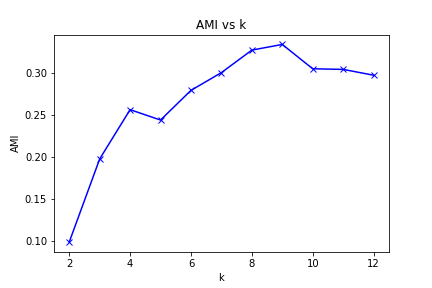
\includegraphics[width=0.8\textwidth] {2_4.png}
\end{center}
}



\end{subquestion}

\begin{subquestion}{\label{Q_CLUSTER_TRENDS}(3 points) Discuss any trends and interesting aspects which emerge from the plot. Does this follow from your expectations?}



\answerbox{10em}{
The AMI increases as the number of clusters increase from 2 to 8 clusters. 4 Clusters seems to be interesting as the AMI is higher than that for 5 Clusters. The AMI is highest at 9 clusters. The AMI decreases for clusters 10, 11, 12. Ideally we would expect 8 Clusters to have the highest AMI. However, this is very close as the highest AMI is at 9 clusters. A high AMI means that the predicted classes were closer to the true values. The drop in AMI after 9 clusters is also as expected as the true values of class labels only range from 0 to 7.
}



\end{subquestion}

\begin{subquestion}{\label{Q_CLUSTER_FOUR}(6 points) Let us investigate the case with four (4) clusters in some more detail. Using seaborn's \href{https://seaborn.pydata.org/generated/seaborn.countplot.html}{\texttt{countplot}} function, plot a bar-chart of the number of data-points with a particular class (encoded by colour) assigned to each cluster centre (encoded by position on the plot's x-axis). As part of the cluster labels, include the total number of data-points assigned to that cluster.}



\answerbox{40em}{
\begin {center}
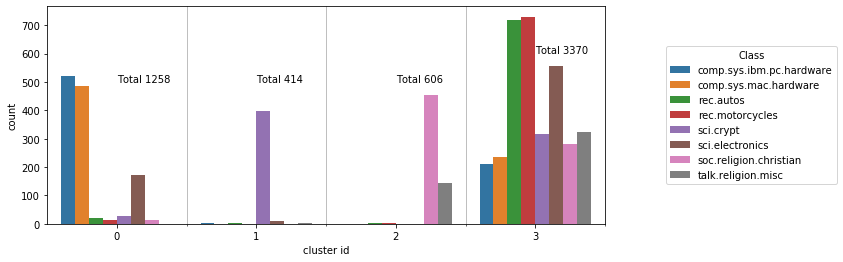
\includegraphics[width=1\textwidth] {2_6_1.png}
\end{center}
}



\end{subquestion}

\begin{subquestion}{(3 points) How does the clustering in Question\ref{Q_UNSUP_LEARN}:\ref{Q_CLUSTER_FOUR} align with the true class labels? Does it conform to your observations in Question\ref{Q_UNSUP_LEARN}:\ref{Q_CLUSTER_TRENDS}?}



\answerbox{14em}{
The clustering separates the sci.crypt as it is the only one with a dominant peak. However, the other data points are not well separated. The true class labels do not align with the predicted labels. This conforms to observations of AMI in Q2.5 as the AMI is low (AMI for n\_clusters = 4 is 0.24) i.e low similarity between true and predicted labels.
}



\end{subquestion}



\end{question}

%============================================================================%

\begin{question}{(26 points) Logistic Regression Classification}
\label{Q_LR_NG}
\questiontext{We will now try out supervised classification on this data. We will focus on Logistic Regression and measure performance in terms of the \href{https://scikit-learn.org/stable/modules/generated/sklearn.metrics.f1_score.html}{F1} score (familiarise yourself with this score which is related to the precision and recall scores that we learnt about in class).}



\begin{subquestion}{(3 points) What is the F1-score, and why is it preferable to accuracy in our problem? How does the macro-average work to extend the score to multi-class classification?}



\answerbox{8em}{
F1 Score = 2*((Precision*Recall)/(Precision+Recall)). It is more preferable to accuracy as False Negatives/Positives are important in our problem. Accuracy can be largely contributed to by a high number of True Positives/Negatives which is not useful in our problem. Macro average calculates the F1 separated by class.
In multi-class classification the macro average is heavily penalized if the classifier performs badly in these classes with lower number of samples.
}

\end{subquestion}


\begin{subquestion}{(2 points) As always we start with a simple baseline classifier. Define such a classifier (indicating why you chose it) and report its performance on the \textbf{Test} set. Use the `macro' average for the \texttt{f1\_score}.} %\hint{For the baseline, the classifier should use only the target labels.}



\answerbox{8em}{
The sklearn DummyClassifier with stratified strategy gives a f1-score macro avg of 0.1283.

The stratified Dummy Classifier predicts that there is a 90\% probability that each object it encounters possesses the target property. The most frequent strategy would not be as useful because most of the classes have a similar size.
}



\end{subquestion}

\begin{subquestion}{(3 points) We will now train a \href{https://scikit-learn.org/stable/modules/generated/sklearn.linear_model.LogisticRegression.html}{LogisticRegression} Classifier from SKLearn. By referring to the documentation, explain how the Logistic Regression model can be applied to classify multi-class labels as in our case. \hint{Limit your explanation to methods we discussed in the lectures.}}



\answerbox{9em}{
The SKLearn Logistic Regression Classifier in the multi\_class mode can be set to use the one vs rest (OvR) scheme (multi\_class='ovr'). This will fit a binary problem for each of the class labels in our data-set. i.e Creates different weight vectors $wk$ for each class to classify into k and not-k. In order to classify a new input the Linear Regressor maximizes the probability that it belongs to a certain class.
}



\end{subquestion}

\begin{subquestion}{(4 points) Train a Logistic Regressor on the training data. Set \texttt{solver=`lbfgs'}, \texttt{multi\_class=`multinomial'} and \texttt{random\_state=0}. Use the Cross-Validation object you created and report the average validation-set F1-score as well as the standard deviation. Comment on the result.}



\answerbox{9em}{
The average-validation-set F1 score is 0.67 

The Standard Deviation is 0.0135

The logistic regressor F1 score is approximately 5 times the baseline regressor F1 score. The standard deviation is small which suggests a tight spread of data around the mean.
}



\end{subquestion}

\begin{subquestion}{\label{Q_LOG_REG_PLT}(5 points) We will now optimise the Regularisation parameter $C$ using cross-validation. Train a logistic regressor for different values of $C$: in each case, evaluate the F1 score on the training and validation portion of the fold. That is, for each value of $C$ you must provide the training set and validation-set scores per fold and then compute (and store) the average of both over all folds. Finally plot the (average) training and validation-set scores as a function of $C$. \hint{Use a logarithmic scale for $C$, spanning 19 samples between $10^{-4}$ to $10^5$.}}



\answerbox{40em}{
\begin {center}
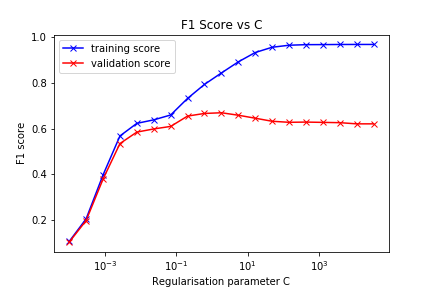
\includegraphics[width=1\textwidth] {3_5.png}
\end{center}
}



\end{subquestion}

\begin{subquestion}{(7 points) What is the optimal value of $C$ (and the corresponding score)? How did you choose this value? By making reference to the effect of the regularisation parameter $C$ on the optimisation, explain what is happening in your plot from Question \ref{Q_LR_NG}:\ref{Q_LOG_REG_PLT} \hint{Refer to the documentation for $C$ in the \href{https://scikit-learn.org/stable/modules/generated/sklearn.linear_model.LogisticRegression.html}{LogisticRegression} page on SKLearn}.}



\answerbox{11em}{
Optimal C = 1.832981 with f1-score = 0.6696. This value of C gives the highest f1-score on the validation set.It is also the point where the over-fitting just starts to become more noticeable. Therefore, it is the point that provides a good balance. In the plot, as the Regularization Parameter C increases, the regularization strength decreases. This means that the model is more likely to over-fit. This can be seen in the graph as the difference in f1 score between the validation set and the training set also increases. The f1- score on the training set is much larger than the f1- score on the validation set for large values of C.
}



\end{subquestion}

\begin{subquestion}{(2 points) Finally, report the score of the best model on the test-set, after retraining on the entire training set (that is drop the folds). \hint{You may need to set \texttt{max\_iter = 200}.} Comment briefly on the result.}



\answerbox{7em}{
The Best Model F1 Score = 0.671 using the value of C identified in the previous question.

The F1 score is very close to the F1-Score using Cross Validation. It is reasonably high for the purpose of our data set.
}



\end{subquestion}


\end{question}




%============================================================================%




%%%%%%%%%%%%%%%%%%%%%%%%%%%%%%%%%%%%%%%%%%%%%%%%%%%%%%%%%%%%%%%%%%%%%%%%%%%%%%
%============================================================================%
%%%%%%%%%%%%%%%%%%%%%%%%%%%%%%%%%%%%%%%%%%%%%%%%%%%%%%%%%%%%%%%%%%%%%%%%%%%%%%

\clearpage

\assignmentSection{Part B: Bristol Air-Quality [90 points]}




\begin{question}{\label{Q_EXPLORATORY}(30 Points) Exploratory Analysis}

\questiontext{We will begin by exploring the Dataset to familiarise ourselves with it.}



\begin{subquestion}{(6 points) Summarise the key features/observations in the data: describe the purpose of each column and report (briefly) also on the dimensionality/ranges (ballpark figures only, and how they compare across features) and number of sites, and identify anything out of the ordinary/problematic: \ie look out for missing data and negative values. Why are the latter unreasonable in such a dataset? \hint{Refer to the documentation for how to interpret the pollutant values.}}



\answerbox{13em}{
Number of instances of training data: 1306758, number of attributes: 7 - 
Date Time: The Date and time on which the data was collected. - 
NOx, NO2, NO: concentration of NOx in the Air.
SiteID: A number that identifies the Site. - 
Loc.Lat, Loc.Long: The latitide \& longitude of the location of the Sites respectively. - 
The Number of Sites is 18. The Date ranges from 1993-01-01 00:00 to 2019-08-12 09:00	
The number of Missing data are: NOx  115538 - NO2  118332 - NO  109222
No data is missing for the other columns.
The concentration of NOx, NO2 and NO can not be negative as it is the measure of mass in unit volume.
However, the following show the number of values for the columns that are negative: NOx 85 - NO2 98 - NO 542
The number of rows which have at least one missing data or negative value are 119445
}



\end{subquestion}

\begin{subquestion}{(6 points) Repeat the same analysis but this time on a per-site basis. Provide a table with the number of samples and percentage of problematic samples (negative and missing) in each site. To report numbers, count a row which has at least one missing entry
as having missing data, and similarly for negative entries. \hint{Pandas has a handy method, \texttt{to\_latex()}, for generating a latex table from a dataframe.}}



\answerbox{17em}{
\scriptsize
\vskip-0.4cm
\begin{tabular}{lrrr}
\toprule
{} &  Number of Samples &  Negative Values (\%) &  Missing Values(\%) \\
SiteID &                    &                      &                    \\
\midrule
0      &               6446 &                  0.00 &               1.61 \\
1      &             163111 &                  0.00 &               6.29 \\
2      &              62990 &                 0.00 &               4.34 \\
3      &              25464 &                 0.77 &              77.33 \\
4      &              74787 &                 0.00 &               2.06 \\
5      &             113952 &                  0.00 &               8.82 \\
6      &             142141 &                 0.00 &               7.44 \\
7      &             115162 &                 0.27 &               4.19 \\
8      &              43824 &                  0.00 &              21.05 \\
9      &              22071 &                  0.00 &               5.30 \\
10     &              96407 &                 0.00 &               3.58 \\
11     &              20693 &                 0.08 &               1.90 \\
12     &              45240 &                  0.00 &              17.48 \\
13     &              12423 &                 0.01 &              51.46 \\
14     &             113951 &                  0.00 &              10.53 \\
15     &               2712 &                  0.00 &             100.00 \\
16     &             154331 &                 0.01 &               6.53 \\
17     &              91053 &                 0.00 &               6.27 \\
\bottomrule
\end{tabular}
}



\end{subquestion}

\begin{subquestion}{(4 points) Briefly summarise how the sites compare in terms of number of samples and amount of problematic samples.}



\answerbox{11em}{
The least number of samples is 2712 for Site Id 15 with 100\% of the samples being problematic. The highest number of samples is 163111 for Site Id 3 with 6.29\% of the samples being problematic. The number of samples ranges from 2712 samples to 163111 samples with mean 72597 samples and standard deviation 53065. Site Id 3,8,13 and 15 have more than 20\% problematic samples. Site ID 13 has more than 50\% problematic samples. The high standard deviation shows that the distribution of samples will be heavily skewed.
}



\end{subquestion}

\begin{subquestion}{(3 points) Given that the columns are all oxides of nitrogen and hence we expect them to be related, we will now look at correlations in our data. This will also be useful in determining how well we can predict any one of the readings from the other two. Remove the data from sites 3 and 15 and compute the \textbf{Pearson} correlation coefficient between each of the three pollutant columns on the remaining data. Visualise the coefficients between each pair of columns in a table.}



\answerbox{10em}{
\begin{tabular}{lrrr}
\toprule
{} &    NOx &    NO2 &     NO \\
\midrule
NOx &  1.000 &  0.878 &  0.988 \\
NO2 &  0.878 &  1.000 &  0.807 \\
NO  &  0.988 &  0.807 &  1.000 \\
\bottomrule
\end{tabular}
}



\end{subquestion}

\begin{subquestion}{(2 points) Comment on the level of correlation between each pair of pollutants.}



\answerbox{7em}{
NOx and NO have the highest positive correlation with pearson correlation co-efficient = 0.988 NOx and NO2 have the second highest positive correlation with pearson correlation co-efficient = 0.878 NO and NO2 have the third highest positive correlation with pearson correlation co-efficient = 0.807. In general, the correlation between each pair is high and is sufficient in order to predict missing values.
}



\end{subquestion}



\begin{subquestion}{\label{CORRELATIONS}(5 points) For each of the three pollutants, compute the Pearson correlation between sites. \hint{You will need to remove the `Date Time' column and then group by the first level of the columns.} Then plot these as three heatmaps: show the values within the figures. \hint{Use the method \texttt{plot\_matrix()} from \texttt{mpctools.extensions.mplext}.}}



\answerbox{40em}{
\begin {center}
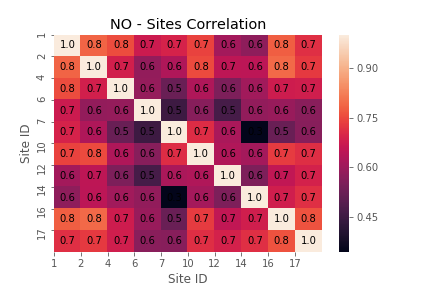
\includegraphics[height=0.35\textwidth] {4_6_1.png}
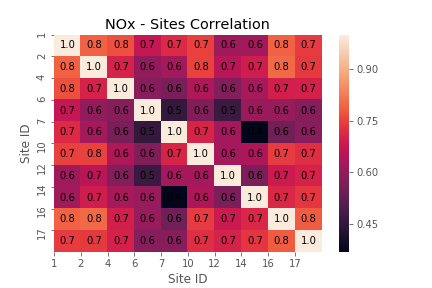
\includegraphics[height=0.35\textwidth] {4_6_2.png}
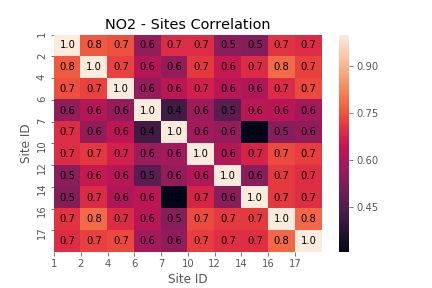
\includegraphics[height=0.35\textwidth] {4_6_3.png}
\end{center}
}



\end{subquestion}

\begin{subquestion}{(4 points) Comment briefly on your observations from Question \ref{Q_EXPLORATORY}:\ref{CORRELATIONS}: start by summarising the results from the NO gas and then comment on whether the same is observed in the other gases or if there is something different.}



\answerbox{12em}{
For NO gas the lowest correlation (0.35) is between site 7 and site 14.

Site 6 has poor correlation (0.45) with Site 7 and Site 12.

All other pairs of Sites have correlation greater than 0.50.

In particular Site 1,2,16 \& 17 have relatively high correlated with each other and most of the other sites.

These patterns are seen strongly in gas NOx and more so in gas N02
}



\end{subquestion}

\end{question}


%============================================================================%

\begin{question}{(19 Points) Principal Component Analysis}

\questiontext{One aspect which we have not yet explored is the temporal nature of the data. That is, we need to keep in mind that the readings have a temporal aspect to them which can provide some interesting insight. We will explore this next.}



\begin{subquestion}{(1 point) Plot the first 5 lines of data (plot each row as a single line-plot).}



\answerbox{40em}{
\begin {center}
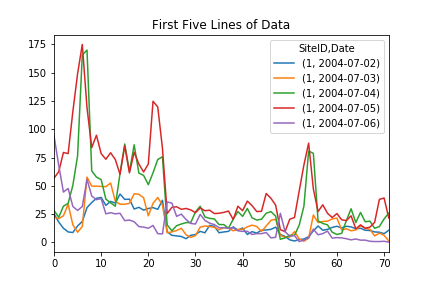
\includegraphics[width=0.9\textwidth] {5_1.png}
\end{center}
}



\end{subquestion}



\begin{subquestion}{(5 points) We will focus first on data solely from Site 1. Extract the data from this site, and run PCA with the number of components set to 72 for now. Set the \texttt{random\_state=0}. On a single graph plot: (i) the percentage of the variance explained by each principal component (as a bar-chart), (ii) the cumulative variance (line-plot) explained by the first $n$ components: (\hint{you should use \href{https://matplotlib.org/3.1.1/api/_as_gen/matplotlib.axes.Axes.twinx.html}{\texttt{twinx()}} to make the plot fit}), \textsl{and}, (iii) mark the point at which the number of components collectively explain at least 95\% of the variance (using a vertical line). \hint{Number components starting from 1.}}



\answerbox{40em}{
\begin {center}
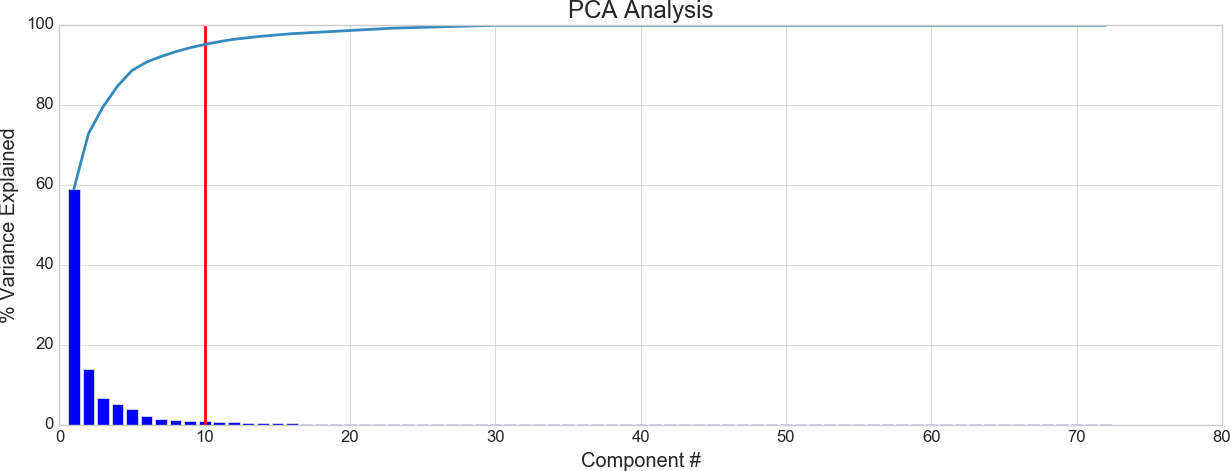
\includegraphics[width=1\textwidth] {5_2.png}
\end{center}
}



\end{subquestion}

\begin{subquestion}{(2 points) Interpret and summarise the above plot.}



\answerbox{9em}{
The above plot shows us the number of components that will be sufficient to explain 95\% of the data using PCA.
The bar chart gives the contribution of each component and the cumulative chart takes their cumulative sum.
The red line at Component \# = 10 means that 10 components are sufficient in order to explain 95\% of the data.
The \% Variance Explained by each component decreases drastically as the component number increases.
}


\end{subquestion}


\begin{subquestion}{(5 points) Generate three figures, one for the mean and one for each of the first 2 principal components: in each, plot the mean/component as three lines, one for each pollutant through one day cycle. \hint{You will need to reshape the components appropriately.}}



\answerbox{50em}{
\begin {center}
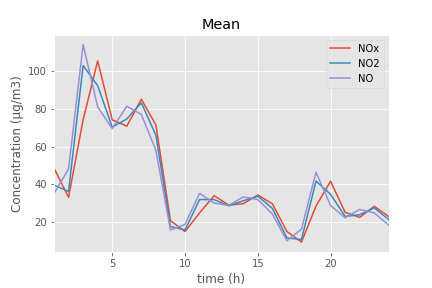
\includegraphics[height=0.28\textheight] {5_4_1.png}
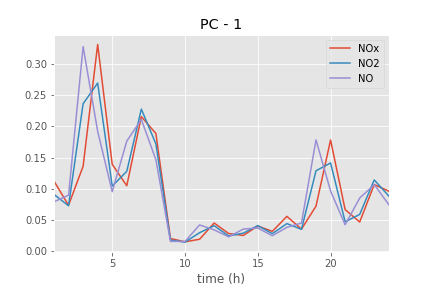
\includegraphics[height=0.28\textheight] {5_4_2.png}
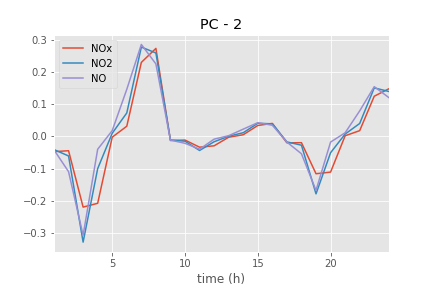
\includegraphics[height=0.28\textheight] {5_4_3.png} 
\end{center}
}



\end{subquestion}

\begin{subquestion}{(6 points) Focusing on the mean and first principal component, are there any significant patterns which emerge throughout the day? \hint{Think about car usage throughout the day.} What is different when interpreting the mean versus the first component? \hint{Do peaks signify the same thing in both cases?} Looking at the principal components only, are there any significant differences between the pollutants? Why could this be happening? \hint{You can refer to one of the limitations of PCA.}}



\answerbox{16em}{
For all three pollutants the pattern through the day is very simmilar for both the mean and the first Principal Component. Both the mean and the first Principal Component have a highest peak in hour 3. They also have a second highest peak in hour 7. Moreover, at around hour 9 both drop significantly in magnitude. In the following hours both have small varations in magnitude until hour 19 where they have their third highest peak. 

The peak of the mean-pc signifies the highest average concentration of the pollutants, whereas the peak of the first pc siginifies the highest variation in concentration of the pollutants.

Thoughout the day, all three polutant concentrations vary in the same pattern. The differences could be due to the different proprotions in which NO, NO2 and NOx are present in the air.
}



\end{subquestion}

\end{question}

%============================================================================%


\begin{question}{\label{Q_LR_BA}(41 points) Regression}


\questiontext{Given our understanding of the correlation between signals and sites, we will now attempt to predict the NOx level for Site 17 given the value at the other sites. We will evaluate our models using the Root Mean Squared Error (RMSE) \ie the square root of the \href{https://scikit-learn.org/stable/modules/generated/sklearn.metrics.mean_squared_error.html}{mean\_squared\_error} score by sklearn.}



\begin{subquestion}{(2 points) First things first: since we are dealing with a supervised task, we will need to split our data into a training and testing set. Furthermore, since some of our regressors will involve hyper-parameter tuning, we will also need a validation set. Use the \texttt{multi\_way\_split()} method from \texttt{mpctools.extensions.skext} to split the data into a Training (60\%), Validation (15\%) and Testing (25\%) set: use the \href{https://scikit-learn.org/stable/modules/generated/sklearn.model_selection.ShuffleSplit.html}{ShuffleSplit} object from sklearn for the \texttt{splitter}. Set the random state to 0. \hint{The method gives you the indices of the split for each set, which can then be applied to multiple matrices.} Report the sizes of each dataset.}



\answerbox{4em}{
training set size: 8937 --- validation set size: 2234 --- testing set size: 3724
}



\end{subquestion}

\begin{subquestion}{(4 points) Let us start with a baseline. By using only the $y$-values, what baseline regressor can you define (indicate what it does)? Implement it and report the RMSE on the training and validation sets. Interpret this relative to the statistics of the data.}



\answerbox{8em}{
Using only y-values and always predicting the median of the y-values, the RMSE are the following:
    
RMSE on training set = 82.1 - RMSE on validation set = 82.2

Std of training y-values = 79.7 - Std of validation y-values = 80.2 

The RMSE values are close to the standard deviation of the y-values which means that our baseline regressor is nearly the equivalent of randomly guessing y-values.
}



\end{subquestion}

\begin{subquestion}{(3 points) Let us now try a more interesting algorithm: specifically, we will start with \href{https://scikit-learn.org/stable/modules/generated/sklearn.linear_model.LinearRegression.html}{LinearRegression}. Train the regressor on the training data and report the RMSE on the training and validation set, and comment on the relative performance to the baseline.}



\answerbox{7em}{
RMSE on training set = 39.8

RMSE on validation set = 41.1

The Linear Regressor is significantly better than the baseline regressor, as it nearly halves the RMSE of the baseline regressor for both the validation set and the training set.
}



\end{subquestion}



\begin{subquestion}{(5 points) We want to explore further what the model is learning. Explain why in Linear Regression, we cannot just blindly use the weights of the regression coefficients to evaluate the relative importance of each feature, but rather we have to normalise the features. By referring to the documentation for the \href{http://scikit-learn.org/stable/modules/generated/sklearn.linear_model.LinearRegression.html}{LinearRegression} implementation in SKLearn, explain what the normalisation does and how it helps in comparing features. Will this affect the performance of the Linear Regressor?}



\answerbox{10em}{
If we compare the coefficients blindly then regardless of their relative importance, the coefficients from features with higher mean (and lower std) will always be larger. This is because the scales of these features are not the same. Normalizing the features gives all of them the same mean and standard deviation which makes their coefficients comparable and allows us to find their relative importance. The SKLearn implementation can normalize the regressor by subtracting the mean and dividing by the Euclidean norm. It will not affect the performance.
}



\end{subquestion}

\begin{subquestion}{(5 points) Retrain the regressor, setting \texttt{normalize=True} and report (in a table) the ratio of the relative importance of each feature. Which is the most/least important site? How do they compare with the correlation coefficients for Site 17 as computed in Question \ref{Q_EXPLORATORY}:\ref{CORRELATIONS}, and why do you think that is?}



\answerbox{15em}{

\vskip-0.32cm
\begin{tabular}{lrrrrrrrrr}
\toprule
Site ID &     1 &    2 &     4 &    6 &     7 &    10 &    12 &    14 &    16 \\
\midrule
Relative Importance &  0.11 &  0.0 &  0.13 &  0.0 &  0.05 &  0.07 &  0.12 &  0.09 &  0.16 \\
\bottomrule
\end{tabular}



The most important site is SiteID 16 (14.86\%). The least important site is SiteID 6 with (0.87\%).
The correlation coefficients from q4.6 are not normalized, therefore they are not directly comparable with the coefficients from the normalized linear regressor (the normalized coefficients are much smaller than the pearson coefficients).
However, they do align with each other i.e SiteID 16 has the highest pearson correlation coefficient as well as the highest normalized regression coefficients. SiteID 6 has the least pearson correlation coefficient as well as the least normalized regression coefficients. This is because if the pearson correlation coefficients were normalized they would be the same as the normalized regression coefficients.
}



\end{subquestion}

\begin{subquestion}{(5 points) It might be that with non-linear models, we may get better performance. Let us try to use \href{https://scikit-learn.org/stable/modules/generated/sklearn.neighbors.KNeighborsRegressor.html}{K-Nearest-Neighbours}. Train a KNN regressor with default parameters on the training set and report performance on the training and validation set. \hint{it might be beneficial to set \texttt{n\_jobs=-1} to improve performance.} How does it compare with Linear Regression in terms of performance on both sets? What is a limitation of the KNN algorithm for our dataset?}



\answerbox{8em}{
Linear Regression RMSE on Validation is 41.1 and on Training is 39.8 

KNN Regressor RMSE on Validation is 31.7 and on Training is 32.1 

KNN uses euclidean distance which is sensitive to magnitudes. The features in our data set with high magnitudes weigh more than the features with low magnitudes. This would not be a limitation if we normalize our data. However our data also has high dimmensionality which makes KNN less accurate.
}



\end{subquestion}

\begin{subquestion}{(4 points) The KNN regression allows setting a number of hyper-parameters. We will optimise only one: the number of neighbours to use. By using the validation set, find the optimal value for the \texttt{n\_neighbours} parameter out of the values [2, 4, 8, 16, 32]. Plot the training/validation RMSE and indicate (for example with a line) the best value for \texttt{n\_neighbours}.}



\answerbox{40em}{
\begin {center}
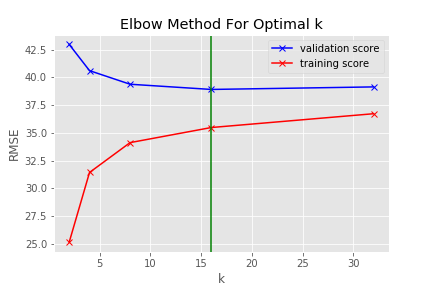
\includegraphics[width=0.95\textwidth] {6_7.png}
\end{center}
}



\end{subquestion}

\begin{subquestion}{(1 points) What is the best-case RMSE performance on the validation set for KNN?}



\answerbox{6em}{
best-case RMSE = 38.9 with n\_neighbors=16
}



\end{subquestion}

\begin{subquestion}{(4 points) Let us try one last regression algorithm: we will now use \href{https://scikit-learn.org/stable/modules/generated/sklearn.tree.DecisionTreeRegressor.html}{DecisionTreeRegressor}. Again, the algorithm contains a number of hyper-parameters, and we will optimise the depth of the tree. Train a series of Decision Tree Regressors, optimising (over the validation set) the \texttt{max\_depth} over the values [2, 4, 8, 16, 32, 64]. Set \texttt{random\_state=0}. Plot the training/validation RMSE and indicate (as before) the best value for \texttt{max\_depth}.}



\answerbox{40em}{
\begin {center}
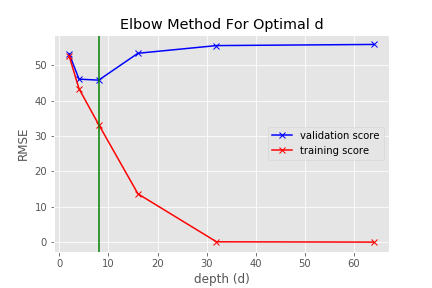
\includegraphics[width=0.95\textwidth] {6_9.png}
\end{center}
}



\end{subquestion}

\begin{subquestion}{(3 points) What is the best-case RMSE performance on the validation set? What do you notice from the plot about the performance of the Decision Tree Regressor?}



\answerbox{6em}{
best-case RMSE = 45.8 with max\_depth=8
The performance of is significantly better on the training set than the validation set. The performance on the validation set decreases after max\_depth=8 i.e the performance decreases as the performance on the training set increases (because the regressor becomes over-fit). 
}



\end{subquestion}

\begin{subquestion}{(5 points) To conclude let us now compare all the models on the testing set. Combine the training and validation sets and retrain the model from each family on it: in cases where we optimised hyper-parameters, set this to the best-case value. Report the testing-set performance of each model in a table \hint{You should have 4 values}.}



\answerbox{6em}{
\begin{tabular}{lllll}
\toprule
{} & Base Line & Linear & Decision Tree & K Neighours \\
\midrule
RMSE      & 80.7      & 40.5   & 43.1          & 38.0\\      
\bottomrule 
\end{tabular}

}



\end{subquestion}

\end{question}

%============================================================================


\end{document}
